%!TEX root=nips_2016.tex
\section{A recurrent neural network for discrete sequences}
In this section we describe how to construct a generative adversarial network (GAN) that is able to generate text from random noise samples. We also give a simple algorithm to train our model, inspired by recent work in adversarial modeling.

\begin{figure*}[t!]
\begin{center}
\centerline{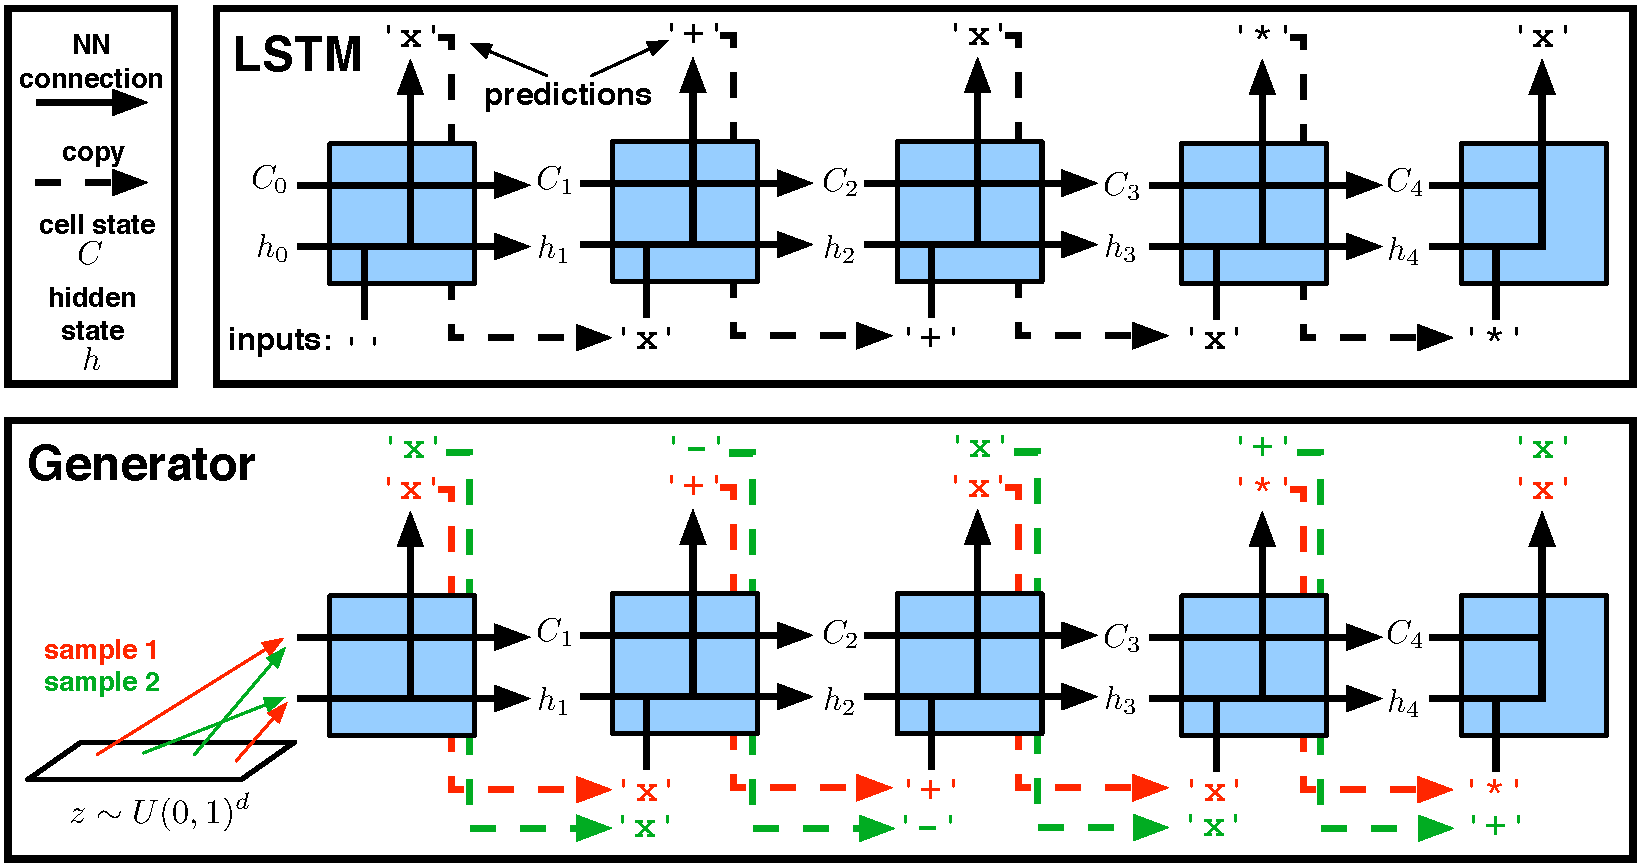
\includegraphics[width=\textwidth]{lstm_gan.pdf}}
%\vspace{-2ex}
\caption{(\emph{Top}): The classic LSTM model during the prediction phase. Each LSTM unit (shown as a blue box) makes a prediction based on the input it as seen in the past. This prediction is then used as input to the next unit, which makes its own prediction, and so on. (\emph{Bottom}): Our generative model for discrete sequences. At the beginning we draw a pair of samples which are fed into the network in place of the initial cell state $C_0$ and hidden state $h_0$. Our trained network takes these samples and uses them to generate an initial character, this generated character is fed to the next cell in the LSTM as input, and so on.}
%\vspace{-5ex}
\label{figure.prediction}
\end{center}
\end{figure*}



Our generative model is based on a Long Short Term Memory (LSTM) recurrent neural network \cite{hochreiter1997long}, shown in the top of Figure~\ref{figure.prediction}. Specifically, an LSTM can be constructed to sequentially predict the next element in a discrete sequence, given the previous elements. Instead, our generative model takes as input a sample-pair which effectively replace the initial cell and hidden states. From this sample our generator constructs a sequence by successively feeding its predictions as input to the following LSTM unit. The immediate difficulty is how to train this generative network to sample realistic sequences.

Given a set of $n$ data points $\{ \x_1, \x_2 \ldots, \x_n\}$ independently and identically drawn from a $d$-dimensional distribution $p(\x)$, the goal of generative modeling is to learn a distribution $q(\x)$ that accuratley approximates $p(\x)$. The framework of generative adversarial modeling has been shown to yield models $q(\x)$ that generate amazingly realistic data points. The adversarial training idea is straight-forward. First, we are going to learn a so-called \emph{generator} $G$ that transforms samples from a simple, known distribution (e.g., a uniform or Gaussian distribution) into samples that approximate those drawn from $p(\x)$. Specifically, we define $q(\x) := G(\z)$, where $\z \sim U(0,1)^d$ (we define $U(0,1)^d$ as the $d$-dimensional )




\begin{figure*}[t!]
\begin{center}
\centerline{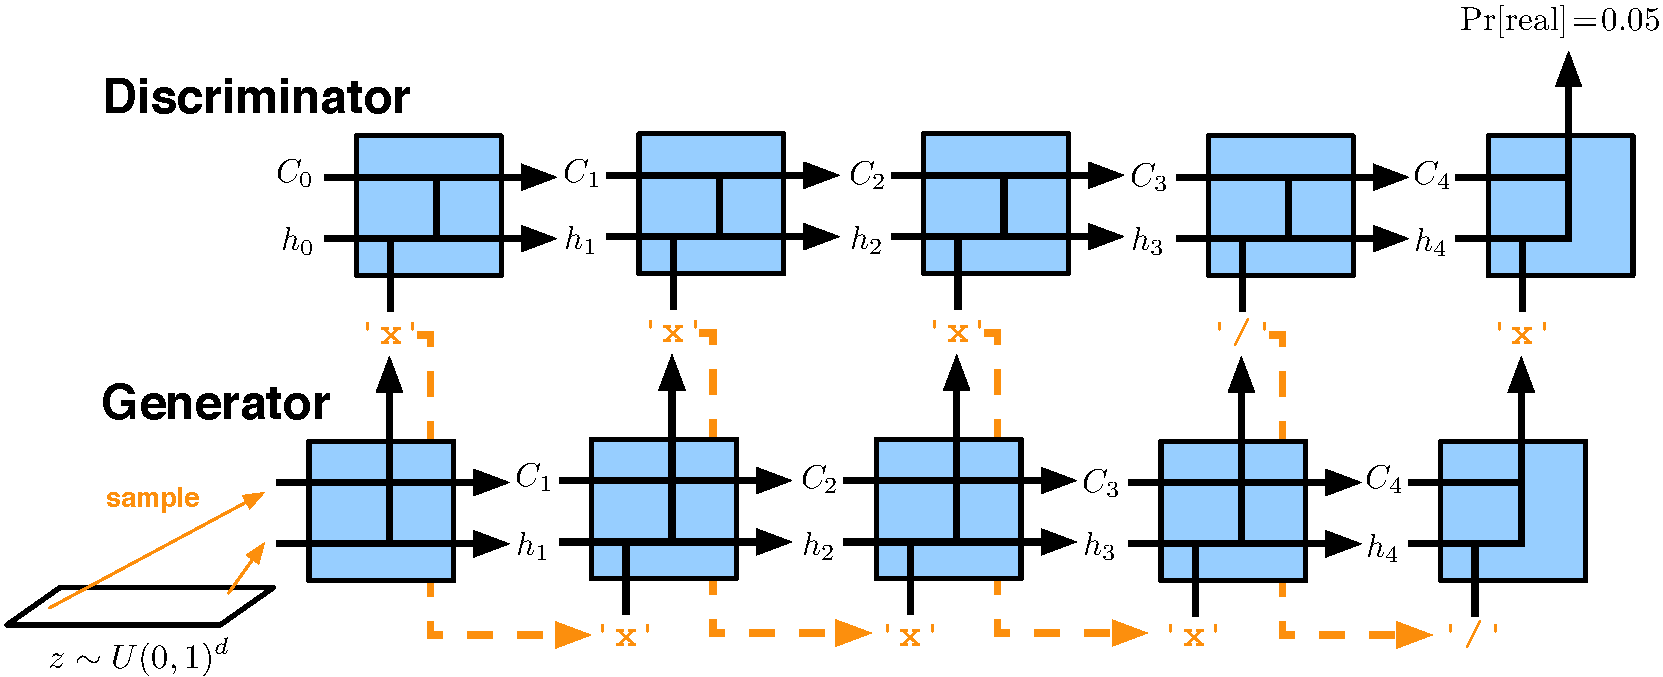
\includegraphics[width=\textwidth]{GAN.pdf}}
%\vspace{-2ex}
\caption{The adversarial training procedure. Our generative model first generates a full-length sequence. This sequence is fed to the discriminator (also a LSTM), which predicts the probability of it being a real sequence. Additionally (not shown), the discriminator is fed real discrete sequence data, which again it predicts the probability of it being real. The weights the networks are modified to make the discriminator better at recognizing real from fake data, and to make the generator better at fooling the discriminator.}
%\vspace{-5ex}
\label{figure.adversarial}
\end{center}
\end{figure*}


TODO:
MLE, samples
1, plot, samples
2, plot, samples
13,plot, samples
19,plot, samples
JUST LSTM


For learning a generative model for discrete sequences


Generating text from MLE LSTM S=10...
x+x+x+x x   x  
x-x-x+x x      
x-x/x*x x x x x
x-x+x-x x x    
x/x/x+x x   x  
x-x-x*x x   x  
x+x-x+x x      
x+x-x-x   x    
x/x-x*x x x    
x*x-x+x x x   x
x/x/x-x x     x
x/x*x-x x x    
x+x/x*x x      
x-x/x/x x x    
x/x*x*x x x    
x/x/x*x x x   x
x-x/x*x   x x x
x-x+x+x x x    
x/x-x+x x x x  
x-x/x/x   x x  




count=1
dis loss=0.735004213271
gen loss=1.56914517581
-x+x***- *xxx  
+*x- -x+*xx*x x
*-x-/*x*xxx    
-x-x/x+x-   -  
  x-x-x+x-x--- 
- +x*x x     x 
-x-x- - -+xx/x 
/+ x  *  *     
x+xx/-/x*x-x   
 x*x*x*x-xx*-  
x--+xxx-x x   -
 +/+x*x x  /+- 
 +x+++x---x/xx 
-x    + *  /   
 --+*-x*x+x- / 
-x-+*x* -+     
--x-x*-*x-x    
* /x- - +x-    
*+x--/x+x/x *  
**+-* xxx x-+  
count=2
dis loss=0.00017594737901
gen loss=8.9916148922
  xxxxx*x-*x+xx
x*-+x x*--x*/*x
x-xxxxx*xx*/xx*
 -x//x*//x*xx/x
 ** -x-xxxx/xx*
/+/x*-xx/*- xxx
  /*x*xx*x*//-x
x/x*x/x xx*xx+x
-/**+xxx-xxxx/x
x//xxxxxx+x*xxx
/-x/+*xxxx-+/-x
 xxxx*x/x*x/xx-
xxxxxx*+*/xxxx+
/xx*-xxx/x*xxx*
 +x/x*x**+*x/x+
 --x** */xxx*x*
*-xxxxx* xxxxx-
/*++x+xxxxx/+x+
x+x-x//+xx**+xx
/xxxx+x+x/xxx+x



count=13
dis loss=1.0772071672
gen loss=1.1372522259
*x+/  +    x*  
x      - -  */ 
 /x     / *    
x+-*x+x-x-x*x+*
+ x *   +      
-          * - 
x  -x*/-x-  -- 
  x///x x  /++ 
-/x/x/x-    -/ 
x//-xxx/x/*/  x
*--x/x*- *-x   
/x  +/-* *     
+ --x*-**/x*x /
+   -   *      
/ -x+/+/+x  /  
 x-x*x/x+x     
x+x   x+   + x 
 +-  +        x
  x-x+x*       
x x        x /-


count=19
dis loss=0.902342276036
gen loss=1.06844680703
x+x//*x   *-   
//- x+/x x /x  
+ *x*x  x x//  
-x+xx//x*//    
/x-x/-  * /    
x/x+/x* - +   *
x//- ///x      
x/x x*x / x  x 
+x*x/x/x     x/
/* x+  x      -
xxx+/x+x/x    +
/x x+x+x*x*x +-
x*-+x/* //x x *
x+x*x *-  x +  
 **x+x-x       
*x*x+x*xx /    
x-x+x-*/x+x+   
*/xx+ x /  x * 
-*+*x x + x+   
++*x x*x   - + 
